% !TEX root = ../../../main.tex
% 来源：中学数学实验教材·第三册（高中数学）
% 章节：任意角的三角函数 / 弧和角的概念及其度量
% 原始文件：6.tex，行 68-85
% 类型：tikz
% ---
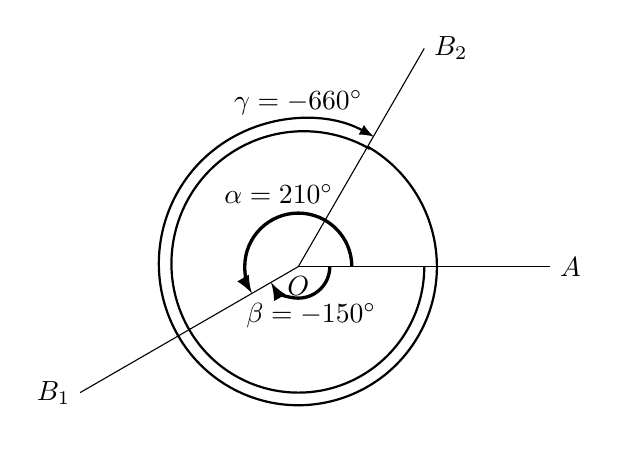
\begin{tikzpicture}[>=latex, scale=.8]
\draw (0,0)node[below]{$O$}--(4,0)node[right]{$A$};
\draw (0,0)--(-150:4)node[left]{$B_1$};    
\draw (0,0)--(60:4)node[right]{$B_2$};    
\draw[->, very thick] (.5,0) arc (0:-150:.5);
\node at (-75:.8){$\beta=-150^{\circ}$};

\draw[->, very thick] (.85,0) arc (0:210:.85);
\node at (105:1.2){$\alpha=210^{\circ}$};

\draw[thick] (2,0) arc (0:-150:2) ;
\draw[thick] (-150:2) arc (-150:-150-150:2.1) ;
\draw[thick] (60:2.2) arc (60:-150:2.2);
\draw[->, thick] (-150:2.2) arc (-150:-150-149:2.3);
\node at (0,2.6){$\gamma=-660^{\circ}$};


\end{tikzpicture}
